\documentclass[12pt,a4paper]{amsart}
% ukazi za delo s slovenscino -- izberi kodiranje, ki ti ustreza
\usepackage[slovene]{babel}
%\usepackage[cp1250]{inputenc}
%\usepackage[T1]{fontenc}
\usepackage[utf8]{inputenc}
\usepackage{amsmath,amssymb,amsfonts}
\usepackage{url}
%\usepackage[normalem]{ulem}
\usepackage[dvipsnames,usenames]{color}
\usepackage{eurosym}
\usepackage{graphicx}

% ne spreminjaj podatkov, ki vplivajo na obliko strani
\textwidth 15cm
\textheight 24cm
\oddsidemargin.5cm
\evensidemargin.5cm
\topmargin-5mm
\addtolength{\footskip}{10pt}
\pagestyle{plain}
\overfullrule=15pt % oznaci predlogo vrstico


% ukazi za matematicna okolja
\theoremstyle{definition} % tekst napisan pokoncno
\newtheorem{definicija}{Definicija}[section]
\newtheorem{primer}[definicija]{Primer}
\newtheorem{opomba}[definicija]{Opomba}

\renewcommand\endprimer{\hfill$\diamondsuit$}


\theoremstyle{plain} % tekst napisan posevno
\newtheorem{lema}[definicija]{Lema}
\newtheorem{izrek}[definicija]{Izrek}
\newtheorem{trditev}[definicija]{Trditev}
\newtheorem{posledica}[definicija]{Posledica}


% za stevilske mnozice uporabi naslednje simbole
\newcommand{\R}{\mathbb R}
\newcommand{\N}{\mathbb N}
\newcommand{\Z}{\mathbb Z}
\newcommand{\C}{\mathbb C}
\newcommand{\Q}{\mathbb Q}


% ukaz za slovarsko geslo
\newlength{\odstavek}
\setlength{\odstavek}{\parindent}
\newcommand{\geslo}[2]{\noindent\textbf{#1}\hspace*{3mm}\hangindent=\parindent\hangafter=1 #2}


% naslednje ukaze ustrezno popravi
\newcommand{\program}{Finančna matematika} % ime studijskega programa: Matematika/Finančna matematika
\newcommand{\imeavtorja}{Žan Jarc} % ime avtorja
\newcommand{\imementorja}{prof.~dr. Damjana Kokol Bukovšek} % akademski naziv in ime mentorja
\newcommand{\imesomentorja}{asist.~dr. Aleš Toman}
\newcommand{\naslovdela}{Finančni instrumenti osnovani na razpršenosti}
\newcommand{\letnica}{2020} %letnica diplome


% vstavi svoje definicije ...




\begin{document}

% od tod do povzetka ne spreminjaj nicesar
\thispagestyle{empty}
\noindent{\large
UNIVERZA V LJUBLJANI\\[1mm]
FAKULTETA ZA MATEMATIKO IN FIZIKO\\[5mm]
\program\ -- 1.~stopnja}
\vfill

\begin{center}{\large
\imeavtorja\\[2mm]
{\bf \naslovdela}\\[10mm]
Delo diplomskega seminarja\\[1cm]
Mentorica: \imementorja \\[0.3cm]
Somentor: \imesomentorja}

\end{center}
\vfill

\noindent{\large
Ljubljana, \letnica}
\pagebreak

\thispagestyle{empty}
\tableofcontents
\pagebreak

\thispagestyle{empty}
\begin{center}
{\bf \naslovdela}\\[3mm]
{\sc Povzetek}
\end{center}
% tekst povzetka v slovenscini
V povzetku na kratko opiši vsebinske rezultate dela. Sem ne sodi razlaga organizacije dela -- v katerem poglavju/razdelku je kaj, pač pa le opis vsebine.
\vfill
\begin{center}
{\bf Angleški naslov dela}\\[3mm] % prevod slovenskega naslova dela
{\sc Abstract}
\end{center}
% tekst povzetka v anglescini
Prevod zgornjega povzetka v angleščino.

\vfill\noindent
{\bf Math. Subj. Class. (2010):} navedi vsaj eno klasifikacijsko oznako -- dostopne so na \url{www.ams.org/mathscinet/msc/msc2010.html}  \\[1mm]
{\bf Ključne besede:} navedi nekaj ključnih pojmov, ki nastopajo v delu  \\[1mm]
{\bf Keywords:} angleški prevod ključnih besed
\pagebreak



% tu se zacne besedilo seminarja
\section{Uvod}
Finančni trg sestavljajo vrednostni papirji, katerih vrednosti se v času spreminjajo. Zaradi spreminjanja vrednosti vsak vrednostni papir ali pa portfelj papirjev ustvarja donose in izgube. Če donos ali izgubo delimo z začetno vrednostjo papirja ali portfelja, temu rečemo donostnost, ki je izražena v odstotkih in je lahko pozitivna ali negativna. Razpršenost donosnosti je lahko večja ali manjša. Standardnemu odklonu porazdelitve donosnosti rečemo volatilnost.\\

Investitorji lahko s pomočjo informacije o volatilnosti potencialne naložbe ugotovijo kako tvegana je njihova investicija. Pri vlaganju v finančno naložbo z nizko volatilnostjo se pričakuje, da bodo donosi investicije morda nizki, vendar precej netvegani, medtem ko nam lahko investicija v finančno naložbo z visoko volatilnostjo prinese višje donose, vendar tudi večje tveganje.\\

Finančni inštrumenti na osnovi volatilnosti so bili zasnovani, da vlagateljem ponudijo možnost, da trgujejo z razpršenostjo in s tem zavarujejo svoj portfelj pred nenadnimi nihaji. V svojem delu diplomskega seminarja se bom posvetil Chicago Board Option Exchange (CBOE) Volatility Indexu ozroma VIX.\\
Indeks VIX je bil razvit za napovedovanje pričakovane volatilnosti in se izračunava s pomočjo nakupnimi in prodajnimi opcijami ameriškega indeksa Standard \& Poor's 500.
\newpage


\section{Indeks Standard \& Poor's 500}
Indeks Standard \& Poor's 500 ali indeks S\&P 500 je pokazatelj stanja na ameriškem finančnem trgu, ki se najpogosteje uporablja.. Prva objava indeksa je bila 4. 3. 1957 s strani družbe S\&P Dow Jones Indices. Pri izračunu indeksa uporabljajoi 500 največjih ameriških podjetij, ki najbolj reprezentativno predstavljajo ameriško gospodarstvo (če je v ameriškem gospodarstvu 20\% industrijskih podjetij, bo tudi v množici podjetij, ki sestavljajo indeks 20\% industrijskih podjetij.)\\
Najbolj znana podjetja, ki so vključena v S\&P 500 so Apple, Alphabet, General Motors, Goldman Sachs,...
Vrednost indeksa se na borznih trgih pojavljajo pod kratico \^{}GSPC, SPX,... 
\subsection{Izračun indeksa S\&P 500}
Indeks S\&P 500 je kapitalsko utežen. To pomeni, da spremembe vrednosti delnic podjetij z višjo tržno kapitalizacijo bolj vplivajo na spremembe vrednost indeksa, kot pa podjetja z nižjo tržno kapitalizacijo. Kapitalsko oteženost opazimo tudi s formule za izračun S\&P 500 indeksa.
$$
S\&P~500 = \sum_{i}^{}\frac{P_i \cdot{} Q_i}{Div},
$$
kjer je $P_i$ cena delnice $i$-tega podjetja in $Q_i$ število razpoložljivih delnic za trgovanje $i$-tega podjeta. Pri izračunu indeksa uporabimo le število delnic, s katerimi se lahko prosto trguje in ne kar celotno tržno kapitalizacijo podjetja, saj se z določenim delom delnic podjeja ne more trgovati, ker so te vezane za nagrajevanje zaposlenih. V primeru podjetja Apple, je tržna kapitalizacija podjetja približno 1059 milijard \$, medtem ko je prosta tržna kapitalizacija podjetja (angl. free-float market capitalization) približno 844 milijard \$. (17. 3. 2020)\\
Zaradi dveh razlogov se pri izračunavi uporablja tudi deljitelj $Div$:
\begin{itemize}
\item če bi samo seštevali proste tržne kapitalizacije podjetij, bi dobili ogromno število,
\item podjetje je lahko iz različnih razlogov odstranjeno iz izračuna indeksa in ga nadomesti primernejše podjetje. Deljitelj poskrbi, da zaradi takih postopkov ne prihaja do velikih spremembe indeksa.
\end{itemize}
 S\&P Dow Jones Indices ne razkriva, kako izračunavajo devisor, vendar lahko podatek o vrednosti devisorja izračunamo samostojno, če poznamo trenutno vrednost indeksa  S\&P 500. Vrednost deljitelja decembra 2019 je bila približno 8,2 milijarde \$.
\newpage
\subsection{Gibanje indeksa S\&P 500 skozi čas}
Na sliki (\ref{Graf 1}) lahko opazimo, je indeks S\&P~500 v obdobju 2004-2019 skoraj vedno rastel, opažena sta samo dva večja padca, finančna kriza leta 2008 in nenadni padec indeksa pozno leta 2018. 
Medtem ko je bil padec leta 2018 kratkotrajen in se je vrednost indeksa vrnila nazaj na vrednosti pred padcem in celo preseglo mejo 3000, pa je finančna kriza pustila veliko dolgotrajnejše posledice, saj se je indeks vrnil na predkrizne vrednosti šele leta 2013, skoraj 5 let po zlomu finančnega sistema.\
Pregled gibanja vrednosti indeksa v zadnjih 15 letih nakazuje, da Standard \& Poor's 500 indeks ni le uporaben za reprezentacijo ameriškega gospodarstva ampak tudi predstavlja dobro dolgoročno investicijo. Direktno v indeks ne moremo investirati, lahko pa izoblikujemo portfelj delnic, ki je ekvivalenten sestavi indeksa. Kupovanje delnic 500 podjetij je drago zato na trgu obstajajo alternative; terminski posli in opcije na vrednosti indeksa S\&P~500.
\begin{figure}[!h]
\centering
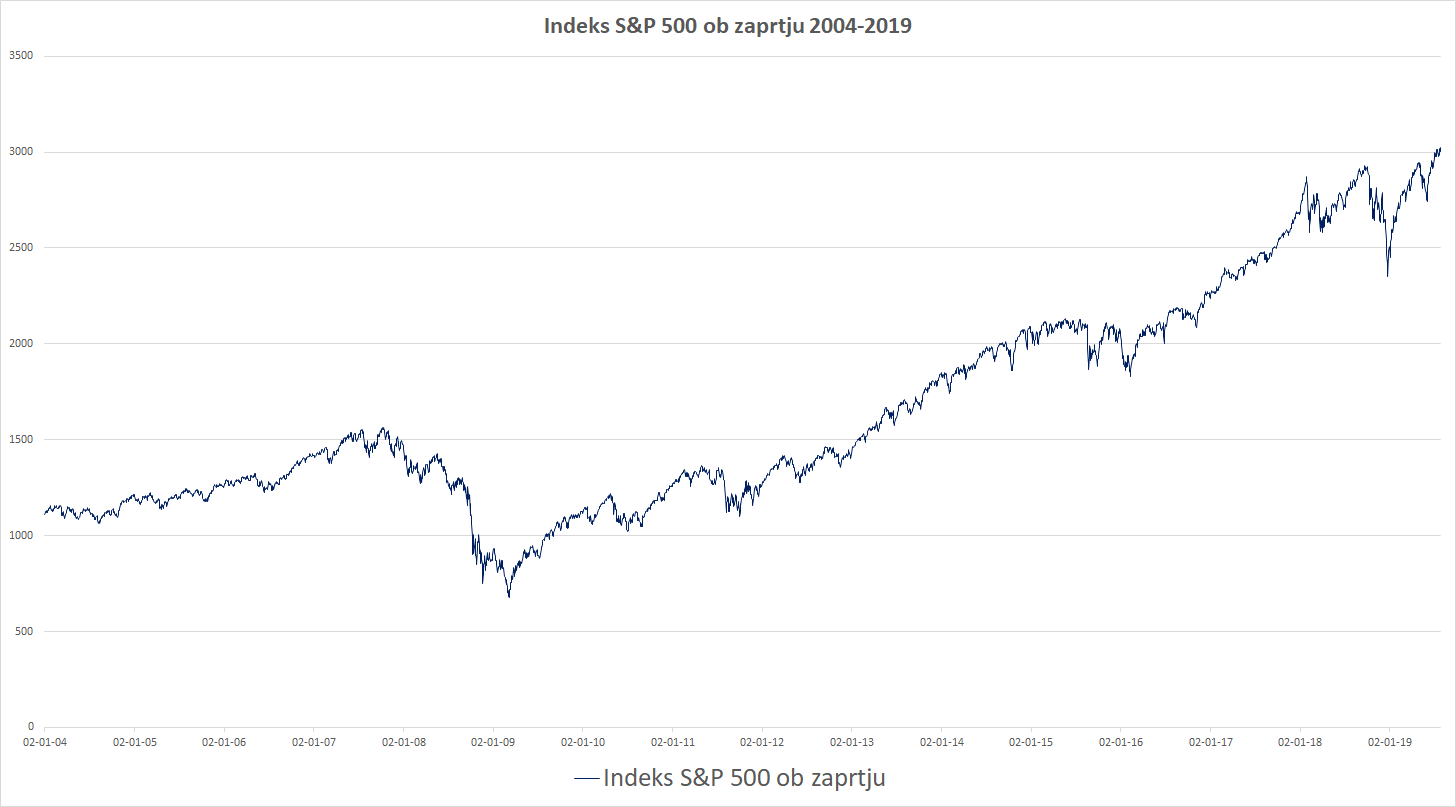
\includegraphics[width = 15 cm]{Grafi/SPX_2004-2019.png}
\caption{Gibanje indeksa S\&P 500 v obdobju 2004-2019, Vir: Yahoo finance}
\label{Graf 1}
\end{figure}


\newpage
\section{Chicago Board Option Exchange Volatility Index}
CBOE Volatility Index ali VIX je bil razvit leta 1993 in se s spremenjeno metodologijo iz leta 2003 uporablja še danes. Indeks prikazuje 30-dnevno pričakovano volatilnost indeksa S\&P 500  in se izračuna s pomočjo nakupih in prodajnih opcij SPX, ki se ne splačajo (out-of-the-money). Da lahko indeks prikazuje res 30-dnevno pričakovano volatilnost, za izračun vzamemo vse prej omenjene opcije, ki zapadejo čez več kot 23 in manj kot 37 dni.\
Indeks s svojimi vrednostmi zelo hitro odraža stanje na trgu in je zato eden najbolj opazovanih indeksov v finančnem svetu.

\subsection{Izračun VIX}
Kot že omenjeno, se pri izračunavi VIX upoštevamo vse nakupne in prodajne opcije na indeks S\&P 500, ki se ne splačajo in zapadejo čez več kot 23 dni in manj kot 37 dni.
Za vsako opcijo določimo njen čas zapadlosti $T$ po formuli:
$$
T = (M_{danasnji\, dan} + M_{dan \,poravnave} + M_{ostali\, dnevi}) / minute\, v\, letu,
$$
kjer je $M_{danasnji\, dan}$ preostalo število minut do polnoči današnjega dneva, $M_{dan \,poravnave}$ je število minut od polnoči do 9:30 ET (US East Coast) za mesečne opcije na indeks S\&P 500 ali pa število minut od polnoči do 16:00 ET za tedenske opcije na indeks S\&P 500, $ M_{ostali\, dnevi}$ pa je število minut preostalih dnevov do zapadlosti posamezne opcije.\\

Za vse opcije, ki zapadejo na isti dan se izračuna za tveganje nevtralna obrestna mera $R$ glede na krivuljo donosa ameriških zakladnih obveznic.\\

Vse opcije, ki zapadejo na isti dan, uredimo po velikosti izvršilne cene in poiščemo tisto opcijo, pri kateri je absolutna razlika med nakupno in prodajno premijo opcije najmanjša. Z izvršilno ceno in nakupno ter prodajno premijo izbrane opcije lahko izračunamo $F$~(forward index level derived from index option prices "prevod?"):
$$
F= Izvrsilna\,cena \cdot e^{R\cdot T} \cdot (Nakupna\, premija - Prodajna\, premija)
$$
Za vsak dan zapadlosti opcij določimo $K_0$, ki je izvršilna cena tiste opcije, ki je enaka ali pa prva manjša od izračunane vrednosti $F$ za tisti dan.\\

Pri izbiri prodajnih opcij, ki bodo uporabljene za izračun indeksa VIX so primerne le tiste z izvršilno ceno manjšo od $K_0,j$. Najprej se izberejo tiste prodajne opcije, ki imajo izklicno ceno takoj pod $K_0$. Nato se nadaljuje iskanje primernih prodajnih opcij z nižjo izvršilno ceno, ki imajo nakupno premijo večjo od 0. Ko se pri iskanju pojavita dve zaporedni opciji z nakupno ceno enako nič se iskanje konča in nobena prodajna opcija z nižjo izvršilno ceno ni vključena za izračun indeksa.\\

Podoben postopek se opravi tudi za iskanje primernih nakupnih opcij, le da se pri tem iskanju upošteva le opcije z izvršilno ceno večjo od $K_0$. V izračun se vključijo najprej tiste nakupne opcije, ki imjao izklicno ceno takoj nad $K_0$ in nato še vse ostalo z višjo izvršilno ceno in nakupno premijo večje od 0. Kot pri izbiri prodajnih opcij, se iskanje nakupnih opcij za izračun indeksa končna, ko se pri razvrščanju naleti na dve zaporedni nakupni opciji, z nakupno premijo enako 0.\\

S tem postopkom so izbrane vse prodajne in nakupne opcije, ki bodo upoštevane pri izračunu indeksa VIX.\\

Za $i-to$ opcijo določimo $K_i$ kot izvršilno ceno izbrane opcije in $\Delta K$ kot:
$$
\Delta K = \frac{K_{i+1} - K_{i-1}}{2}
$$
ter $Q(K_i)$ kot povprečje nakupne in prodajne premije $i-te opcije$.\\

Z izračunanimi vrednostmi za vsak dan izračunamo:
$$
\sigma_j^2 = \frac{2}{T}\sum_{i}{}\frac{\Delta K_i}{K_i^2}e^{RT}Q(K_i) - \frac{1}{T}(\frac{F}{K_0} - 1)^2, \quad \forall j \in {23, 24, \dots, 37}
$$
Za končni izračun indeksa VIX moramo izračunati 30-dnevno uteženo povprečje $\sigma_j^2$:
$$
VIX = 100 \cdot \sqrt{\frac{1}{N_{37}-N_{23}}\Bigg\{ \sum_{j=23}^{37}T_j\sigma_j^2\left\lvert N_j - N_{mesec}\right\rvert \Bigg\}\cdot \frac{N_{leto}}{N_{mesec}}},
$$
kjer je:
\begin{itemize}
\item $N_j$ število minut do zapadlosti opcije, ki zapade čez $j$ dni
\item $N_{leto}$ število minut v letu ($365\cdot1440=525.600$)
\item $N_{mesec}$ število minut v mesecu ($30\cdot1440=43.200$)
\end{itemize}
\newpage
\subsection{Gibanje indeksov VIX in S\&P 500}
Če z grafom primerjamo časovni vrsti vrednosti indeksa S\&P 500 in indeksa VIX(slika \ref{Graf 2}), opazimo, da bo v času rasti indeksa S\&P 500 volatilnost nizka, v času padca pa visoka. Podobno hitro opazimo, če primerjamo vrednosti indeksov VIX in S\&P 500.\

Kot je nazorno razvidno iz grafa \ref{Graf 2} sta indeksa negativno korelirana. \
Negativna korelacija je najbolj opazna v času finančne krize 2008, ko je vrednost indeksa S\&P 500 padla iz 1565,15 oktobra 2008 na 676,53 točke marca 2009, medtem ko je VIX v istem časovnem okvirju zrasel iz 16,12 na 49,68 točke (celo dosegal vrednosti vse do 80,86 točk novembra 2009). \\
Z vlaganjem v VIX, se lahko investitor zavaruje pred nenadnim padcem indeksa S\&P 500 in celotnega ameriškega in svetovnega gospodarstva, vendar direktne investicije v indeks VIX niso možne, saj je le indeks, izračunan z  opcijami na vrednost indeksa S\&P 500, ki se ne izplačajo.\\
Zato obstajajo različni finančni inštrumenti, katerih izplačila so odvisna od vrednosti VIX indeksa, terminski posli na vrednost indeksa VIX in opcije na vrednost indeksa VIX. 
\begin{figure}[!h]
\centering
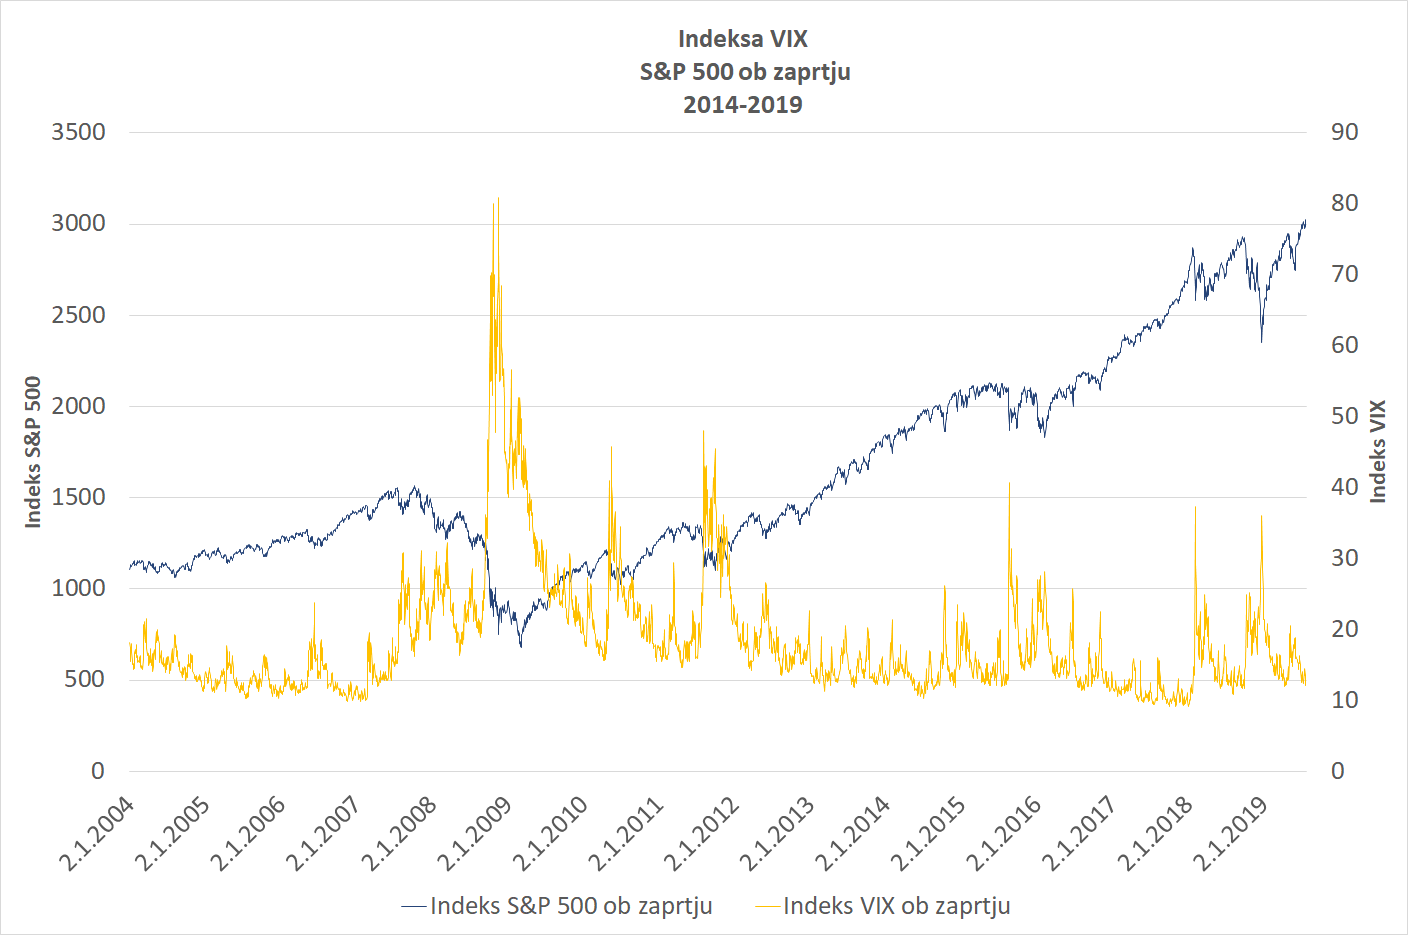
\includegraphics[width = 15 cm]{Grafi/VIX_vs_SPX_2004-2019.png}
\caption{Indeksa VIX in S\&P 500 2004-2019, vir: Yahoo finance}
\label{Graf 2}
\end{figure}
\newpage
\subsection{Terminske pogodbe}
Terminska pogodba (angl. \textit{future}) je izvedeni finančni inštrument, ki zelo natančno določi kaj, kje in za kakšno ceno bo dostavljeno. Za vsako terminsko pogodbo se določi ročnost pogodbe $T$ in izročitveno ceno $K$.\

Čeprav govorimo o prodaji blaga, se terminske pogodbe v večini uporabljajo za investicije. Pri terminski pogodbi bo dolga stran ob ročnosti kupila blago po izročitveni ceno, kratka stran pa jo bo ob ročnosti prodala.\

Če z $S_t$ označimo vrednost premoženja na trgu v času $t$, je z
$$
V_t = S_t - KD(t, T)
$$
označena vrednost terminske pogodbe za kupca (dolgo stran) v času $t$, kjer je $D(t,T)$ diskontni faktor od časa $t$ do časa $T$. 


\subsection{VIX terminske pogodbe}
VIX terminske pogodbe (angl. \textit{VIX futures}) so bili prvič predstavljeni leta 2004 in jih lahko najdemo pod oznako VX (mesečne terminski pogodbe) in VX01 do VX53 (tedenske terminski pogodbe).\

Mesečne terminski pogodbe imajo ročnost na sredo, ki je 30 dni pred petkom, ko zapadajo opcije na vrednost indeksa S\&P 500.\

Vrednosti terminske pogodbe z bližanjem ročnosti konvergirajo k vrednosti VIX. Zaradi tega so kratkoročne terminske pogodbe veliko bolj občutljive na spremembe indeksa VIX, kot pa tiste z daljšo ročnostjo. Pogodbe z daljšo ročnostjo imajo tudi višjo izročitveno vrednost kot pa tiste s krajšo ročnostjo.\

V večini primerov je situacija na trgu stabilna in posledično je indeks VIX nizek in vrednosti terminske pogodbe so višje od vrednosti VIX. Take situacije na trgu se imenujejo \textit{contango}. Če investitor meni, da bo prišlo do spremembe na trgu in s tem dvig vrednosti VIX, sklene dolga pozicija v terminski pogodbi. V primeru negotovosti na trgu in povišanja vrednosti VIX bo imel investitor dobiček, v nasprotnem primeru pa izgubo.\

V primeru, da je trg nestabilen in s tem VIX visok pa so izvršilne vrednosti terminskega posla nižje od vrednosti VIX. Taka stanja se imenujejo \textit{backwardation}.\

Na grafu \ref{Graf 3} je nazorno prikazano obdobje, da so bile vrednosti terminskih pogodb vse do februarja 2018 višje od vrednosti VIX indeksa. S padcem trga pa je indeks VIX narastel in stanje na trgu je prešlo v \textit{backwardation}. Če primerjamo terminski pogodbi za februar in marec 2018, je opazimo, da je bila vrednost marčevske pogodbe do začetka februarja višja od februrarske terminske pogodbe, po šoku na trgu pa je vrednost februrarske terminske pogodbe višja in je bila tudi bolj občutljiva na spremembe VIX kot pa marčevska.
\begin{figure}[!h]
\centering
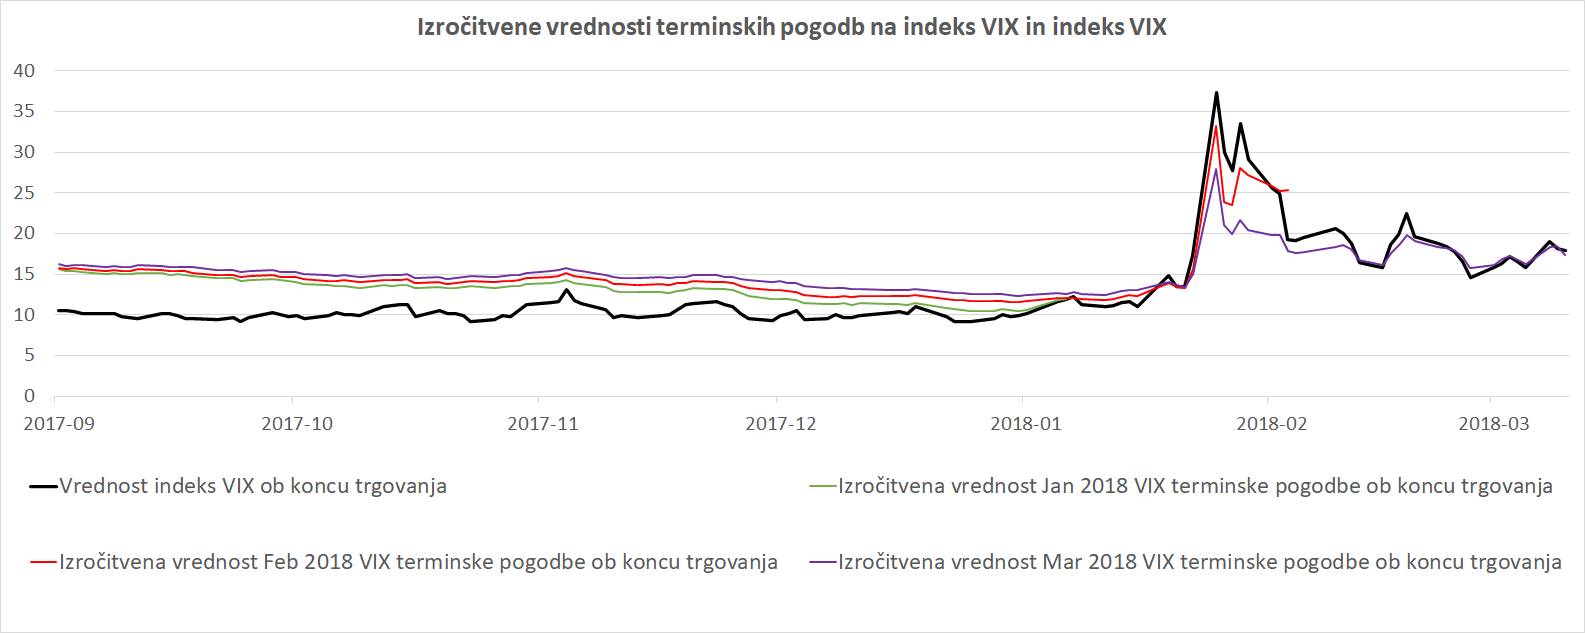
\includegraphics[width = 15 cm]{Grafi/VIX_futures_2018.png}
\caption{Gibanje vrednosti VIX mesečnih terminskih pogodb VIX, vir: Yahoo finance}
\label{Graf 3}
\end{figure}\
\newpage
\subsection{Opcije}
Opcija (angl. \textit{option}) je pogodba podobna terminski pogodbi, s pomembno razlika, da ima kupec opcije pravico se odločiti, ali bo izvršil nakup/prodajo premoženja. Podobno kot pri terminski pogodbi, se pri opciji določi ročnost $T$ in izročitveno ceno $K$.\

Opcije delimo na nakupne opcije in na prodajne opcije. Nosilec nakupne opcije ima pravico se odločiti ali bo kupil premoženje po izročitveni ceni $K$, medtem ko ima nosilec prodajne opcije pravico se odločiti ali bo prodal premoženje po izročitveni ceni $K$.\newline
Kupec ob sklenitvi opcije plača le nakupno/prodajno premijo, potem pa ima le še pravice se odločati.\

Glede na to, kdaj se opcija lahko izvrši, delimo opcije na tri skupine:
\begin{itemize}
\item opcija se lahko izvrši le ob času ročnosti $T$- evropska opcija,
\item opcija se lahko izvrši kadarkoli do vključno časa ročnosti $T$ - ameriška opcija,
\item opcija z drugačnimi pravili - eksotična opcija
\end{itemize}
Pri ameriški opcijami imamo več možnosti in tudi več možnosti za zaslužek. Zato je premija za ameriško opcijo višja kot pa premija za evropsko opcijo.
\subsection{VIX opcije}
VIX opcije (angl. \textit{VIX options}) so bile prvič na voljo leta 2006 in jih najdemo pod kratico VIX. Opcije so evropske in imajo podobno kot terminske pogodbe, ročnost na sredo, ki je 30 dni pred petkom, ko zapadejo opcije na vrednost indeksa S\&P 500.\

Medtem, ko so vrednosti VIX terminskih pogodb neposredno vezane na vrednost indeksa VIX pa so VIX opcije vezane na vrednost terminske pogodbe z enako ročnostjo.
Podobno kot pri terminskih pogodbah se z sklenitvijo nakupne VIX opcije zavarujemo pred šokom na finančnem trgu.
%\section*{Slovar strokovnih izrazov}

% slovar
%\geslo{}{}
%
%\geslo{}{}
%


% seznam uporabljene literature
%\begin{thebibliography}{99}

%\bibitem{}

%\end{thebibliography}

\end{document}

